%File: formatting-instruction.tex
\documentclass{aamas_extabstract}
%\documentclass[letterpaper]{article}

%\documentclass{aamas2013}
\usepackage{epstopdf}
\usepackage{amsfonts}
\usepackage{amsmath}
\usepackage{algorithmicx}
\usepackage{algpseudocode}
\usepackage{algorithm}

%\fontsize{24}{6}
%\selectfont

%\usepackage{draftwatermark}
%\SetWatermarkScale{1}
%\SetWatermarkLightness{.9}
%\SetWatermarkAngle{-45}
%\SetWatermarkText{DRAFT DRAFT DRAFT DRAFT}


%\usepackage[usenames]{color}
\DeclareMathOperator*{\argmin}{argmin}

%\makeatletter
%\let\@copyrightspace\relax
%\makeatother

% if you are using PDF LaTex and you cannot find a way for producing
% letter, the following explicit settings may help

\pdfpagewidth=8.5truein
\pdfpageheight=11truein

\begin{document}

\AuthorsForCitationInfo{William Curran, Adrian Agogino, Kagan Tumer}

%\TitleForCitationInfo{Extending the Difference Reward to Multi-Objective Reinforcement Learning}

%\title{Extending the Difference Reward to Multi-Objective Reinforcement Learning}

\TitleForCitationInfo{Using Reward/Utility Based Impact Scores in Partitioning}
\title{Using Reward/Utility Based Impact Scores in Partitioning}

%\titlenote{For use with aamas2011.cls}}

% AUTHORS

\numberofauthors{3}

\author{
\alignauthor
William Curran\\
       \affaddr{Oregon State University}\\
       \affaddr{Corvallis, Oregon}\\
       \affaddr{curranw@onid.orst.edu}
\alignauthor
Adrian Agogino\\
       \affaddr{NASA AMES Research Center}\\
       \affaddr{Moffet Field, California}\\
       \affaddr{adrian.k.agogino@nasa.gov}
\alignauthor 
Kagan Tumer\\
       \affaddr{Oregon State University}\\
       \affaddr{Corvallis, Oregon}\\
       \affaddr{kagan.tumer@oregonstate.edu}
}

\maketitle


\begin{abstract}
Reinforcement learning with reward shaping is a well-established but often computationally expensive approach to multiagent problems. Agent partitioning can assist in this computational complexity by treating each partition of agents as an independent problem. We introduce a novel agent partitioning approach called Reward/Utility-Based Impact (RUBI). RUBI finds an effective partitioning of agents while requiring no prior domain knowledge, provides better performance by discovering a non-trivial agent partitioning, and leads to faster simulations. We test RUBI in the Air Traffic Flow Management Problem, where there are simultaneously tens of thousands of aircraft affecting the system and no intuitive similarity metric between agents. When partitioning with RUBI in the ATFMP, there is a 37\% increase in performance, with a 510x speed up per simulation step over non-partitioning approaches.

\end{abstract}


\category{I.2.11}{Distributed Artificial Intelligence}{Intelligent Agents}
%\terms{
%Algorithms, 
%Management, 
%Measurement, 
%Documentation, 
%Performance, 
%Design, 
%Economics, 
%Reliability%, 
%Experimentation%, 
%Security, 
%Human Factors, 
%Standardization, 
%Languages, 
%Theory, 
%Legal Aspects, 
%Verification.
%}

\keywords{Multiagent Partitioning, Multiagent Learning}

\section{Introduction}
Two key elements in a multiagent reinforcement learning system is minimizing computation time and maximizing coordination. Reward shaping is a field in multiagent reinforcement learning that focuses on the design of rewards, and has been shown to assist in multiagent coordination. This reward shaping is typically at a large cost to computation time, and in large, highly coupled domains reward shaping quickly becomes computationally intractable. 

Partitioning agents into hierarchies \cite{tumer-holmesparker_ala12} or teams \cite{Curran:2013:AHC:2484920.2485183} speeds up computation time for extremely large domains (approx. 10000-40000 agents) while still using the reward shaping technique without approximation error. In this paper we introduce Reward/Utility-Based Impact (RUBI) scores. RUBI partitions agents by determining the effect of one agent's action on another agent's reward. Using this metric it develops similarity metrics between all agents in order to usefully partition and therefore reduce the complexity of the learning problem. In contrast to many other partitioning approaches, this has the advantage of requiring \textit{no domain knowledge}.

The contributions of this work are: \textbf{Generality}: RUBI requires no prior knowledge of the domain, essentially treating the domain as a black box to obtain rewards from. \textbf{Usability}: RUBI removes the need to derive similarity metrics, removing the need for domain experts in situations where a domain expert isn't available. \textbf{Performance}: RUBI discovers non-trivial agent partitioning by using a reward function to partition agents. \textbf{Speed}: RUBI leads to a larger number of partitions without losing performance, leading to more independence and therefore faster simulations.

%\section{Related Work}

%Previous work in agent partitioning has focused on what specifically to partition. Jordan and Jacobs \cite{716791} developed the Hierarchical Mixtures of Experts (HME) method to partition the state space directly, such that different agents can focus on specific regions of the state space. This method works well in non-linear supervised learning tasks. In this work all learning is unsupervised, so this technique cannot be used.

%Partitioning actions so that each agent is responsible for a small number of actions is another approach used often. Sun and Pearson \cite{Sun98someexperiments} divided actions into two types, speed and turn, and each type was handled by a separate agent. This approach uses domain knowledge, and partitioning actions applies well in robotics, but not in domains where all actions need to be explored.

%The last partitioning technique we describe is to partitioning system-level goals into smaller tasks. In the work by Dayan and Hinton \cite{Dayan93feudalreinforcement}, they accomplished goal partitioning through task allocation, where agents are organized in a hierarchy, where high-level agents assign goals to agents lower in the hierarchy on-line. In the work by Reddy and Tadepalli \cite{Reddy_learninggoal-decomposition}, the approach is more structured. In this work the partitioning of the goal is learned through externally provided examples. Overall, these approaches are under the assumption that the system-level goal can be subdivided, which is not always the case. 

%In this work, we partition agents, essentially treating each partition of agents as an independent problem. Agents from one partition could potentially affect the environment of agents in another partition, but this work attempts to minimize the partition overlap. In a partitioning with complete reward independence, this work essentially treats the problem as a set of smaller and easier independent problems.

%The difference reward function reduces noise from agents in the system \cite{tumer-wolpert_jair02}. This leads to final better policies at an accelerated converge rate. The difference evaluation function is defined as: $D_i(z) = G(z) + G(z - z_i + c)$ where $z$ is the system state, $z_i$ is the system state with agent $i$, and $c$ is a counterfactual replacing agent $i$. This counterfactual offsets the artificial impact of removing an agent from the system.

%In this paper, agents are assigned to one of 35,844 aircraft with cooperation enforced by airport terminals. Aircraft flight plans are from historical flight data from the FAA. Therefore, the only aspect of the environment we can change is the ground delay for each aircraft. Agents may select a certain amount of ground delay from 0 to 10 minutes (11 actions) in the beginning of every simulation. The FAA data has the sector location of each plane for every minute that plane was in service. 

%Agents learned using Action-Value Learning with a zero initialized value table. 

\section{RUBI}

In this work we introduce an autonomous partitioning algorithm requiring no domain knowledge, the Reward/Utility Based Impact algorithm. We develop an initial agent similarity matrix that uses no knowledge about the domain, and partitions agents together based on the impact of one agent to another. This matrix can then be used as an input to a hierarchical agglomerative clustering algorithm. 

If one agent's action heavily impacts another agent's reward, those agents are coupled enough to be partitioned together. The RUBI algorithm computes a localized reward for each agent with agent $i$ in the system, and then compares that reward to the localized reward for each agent if agent $i$ is not in the system. This partitioning algorithm is based around the central idea: $|L_i(z) - L_i(z-z_j)| > |L_k(z) - L_k(z-z_j)| \Rightarrow SIM(i,j) > SIM(k,j)$, where $L_i(z-z_j)$ is the localized reward of agent $i$ if $j$ is not in the system, $L_k(z-z_j)$ is the localized reward of agent $k$ if $j$ is not in the system, and $L_i$ and $L_k$ are the localized rewards of $i$ and $k$ when all agents are in the system. This means that if the localized reward of agent $i$ changes more than the localized reward of agent $k$ when agent $j$ is taken out of the system, agent $j$ has more effect on agent $i$ than agent $k$. 

\textbf{Implementation}: The RUBI algorithm first initializes an $N$ x $N$ matrix $C$, where $N$ is the number of agents within the system. It then calculates actions based on the $ACT()$ function, which is typically random action selection. A simulation is then ran with all of the agents in the system and the localized reward is calculated for every agent. We then remove an agent from the system, recalculate the reward for each agent (since this is a localized reward, this is typically a fast operation), and update the impact table $C$. 
%
\begin{algorithm} [t]\label{alg:RUBI}
  \caption{Reward/Utility Based Impact Algorithm}
  \begin{algorithmic}[1]
    \Statex
    \Function{RUBI}{$sim$}
      \State{$C \leftarrow N x N$}
	  \For{$i \leftarrow 1$ to $iterations$}     
	    \State{$actions \leftarrow ACT()$}
	    \State{$sim.run(actions)$}
	    \State{$L(z) \leftarrow sim.getRewards()$}      
		\For{$r \leftarrow 1$ to $N$}
			\State{$sim.removeAgent(r)$}
			\State{$L(z-z_r) \leftarrow sim.getRewards()$}
			\For{$a \leftarrow 1$ to $N$}
				\State{$C_{r,a} \leftarrow C_{r,a} + |L_a(z) - L_a(z-z_r) |$}
				\EndFor
			\State{$sim.addAgent(r)$}
		\EndFor
	\EndFor        
    \EndFunction
  \end{algorithmic}
\end{algorithm}
%

\textbf{Reward/Utility-Based Impact:} The impact data used to compute the similarity matrix is obtained from a localized reward or utility with respect to an agent. Learning in congestion problems with local rewards typically leads to a poor solution, as agents following local rewards do not optimize the system-level reward. In RUBI, we do not want to learn, but instead analyze the local impact one agent has on another, therefore local rewards are an ideal choice.

RUBI is simply an accumulation of impact scores (line 11 of Algorithm 1). Given enough iterations, this accumulation is informative enough to perform accurate partitioning. In this research we are interested more in the relative impact score from one agent to another, rather than what the explicit impact score is. 

\textbf{Benefits of RUBI:} One of the key strengths of RUBI is its sheer simplicity and generality combined with computing highly informative similarity scores, leading to well-performing partitions. It needs no prior knowledge about the domain to perform partitioning, and simply needs a localized reward from each agent to build the similarity matrix. This makes RUBI highly generic and can be applied to any multiagent domain. 

Additionally, partitions built using RUBI are likely to be greater in number without loss of performance. Domain-based partitioning based on agent similarity encodes how often two agents impact each other. RUBI on the other hand looks more into how the actions of one agent impact another agents reward. If over a few thousand trials the reward impact of two agents is always 0, those agents actions never impact each others reward. The same is true if the reward impact is always the same non-zero value, the actions do not affect the reward, therefore they are not partitioned. This is a key feature of RUBI, and leads to finding more partitions without loss of performance.

\section{RUBI Performance in the ATFMP}
We test RUBI in the Air Traffic Flow Management Problem (ATFMP). The approach used here is the same as in Curran et al. \cite{Curran:2013:AHC:2484920.2485183} and Agogino and Rios \cite{Agogino:2009:EEM:1570256.1570258,Rios}, except utilizing RUBI.

The system-level reward in the ATFMP focuses on the cumulative delay ($\delta$) and congestion ($C$) throughout the system: $G(z) = -(C(z) + \delta(z))$. Agogino and Rios originally had the idea of adding a greedy scheduler to algorithmically remove congestion from the system, while simultaneously using learning to minimize delay. We follow this approach, and therefore our system-level reward is simply: $G(z) = -\delta(z)$

With so many agents, tens of thousands of actions simultaneously impact the system, causing the reward for a specific agent to become noisy with the actions of other agents. A difference reward shaping function reduces much of this noise, and is easily derived from the system-level reward: $D_i(z) = \delta(z-z_i + c_i) - \delta(z)$, where \textit{$\delta(z-z_i + c_i)$} is the cumulative delay of all agents with agent $i$ replaced with counterfactual \textit{$c_i$}. Without RUBI, this reward shaping technique makes the ATFMP computationally intractable.

Partitions developed using RUBI uses similarity metrics that encapsulated the agent coupling. Partitioning with RUBI and the difference reward outperformed the greedy scheduler. Figure \ref{ATFMPNewvsGreedy} shows a variety of partitions out performing the greedy scheduler. The key benefit of RUBI-based partitioning was that a reward independent partition involved 61 partitions, but in domain-based partitioning the smallest was 3. This leads to a 10\% faster processing time, at no cost to performance and using no domain knowledge.

\textbf{Acknowledgments:} This work was partially  supported by the National Science Foundation  under Grant No. CNS-0931591.
%During preliminary analysis, RUBI works as expected in simple toy problems, but what happens when we apply it in a complex domain with tens of thousands of agents, such as the ATFMP? When RUBI is applied during partitioning in the ATFMP, simulation time decreases and the ease of application raises over developing a similarity metric. The removal of domain knowledge allows the same RUBI algorithm to be used in simple problems as well as the ATFMP with no effort and without any need to develop a similarity metric.

%Partitions developed using RUBI uses similarity metrics that encapsulated the agent coupling. In this section we will first show how RUBI partitioning works well in the ATFMP, and analyze the cost/benefit of varying the number of partitions. We will then compare RUBI-based partitioning to domain-based partitioning and see that RUBI develops better quality partitions as well as partitions that lead to faster simulation times.
%
\begin{figure}
\centering
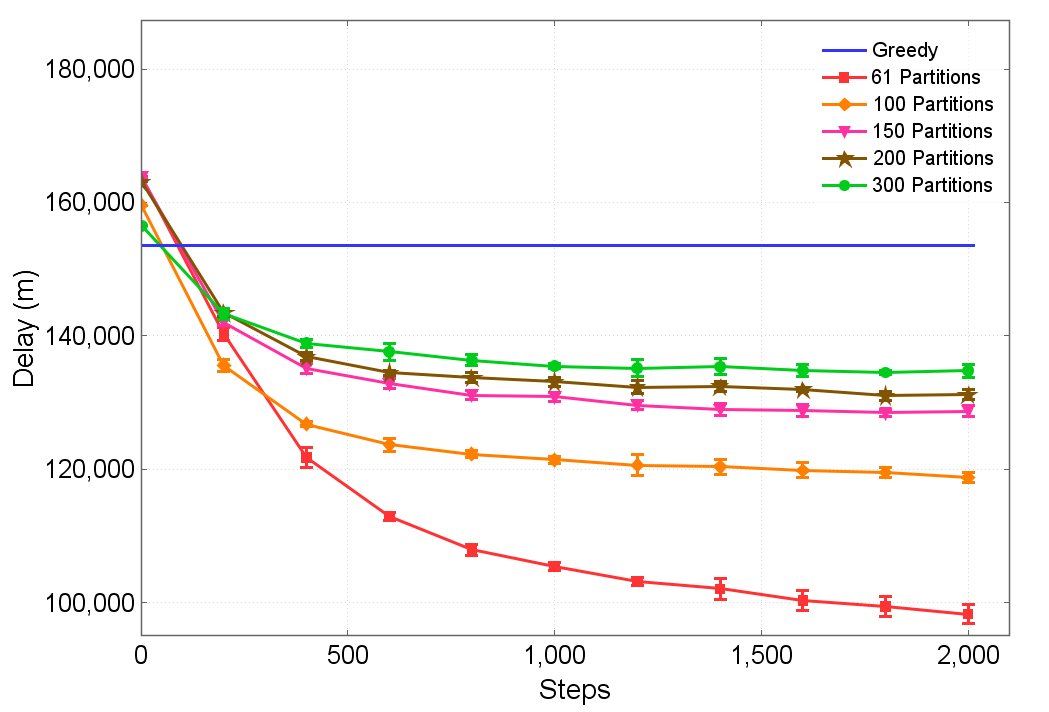
\includegraphics[width=0.75\columnwidth]{ATFMPNewvsGreedy.eps}
\caption{As the number of partitions decreases, performance improves while time complexity increases.}
\label{ATFMPNewvsGreedy}
\end{figure}
%

%When partitioning agents using RUBI in the ATFMP agents took random actions, the greedy scheduler was not used, and the localized reward for each agent involved both congestion and delay (Equation \ref{eq:RUBI ATFMP-L}). The reward-based impact function included both delay and congestion, since the greedy scheduler was removed, so the difference in delay was constantly 0 when computing reward-based impact. Therefore, agents were partitioned together based on whether their actions cause congestion to other agents. 

%Partitioning with RUBI and the difference reward outperformed the greedy scheduler. Figure \ref{ATFMPNewvsGreedy} shows a variety of partitions out performing the greedy scheduler. The final performance of the ATFMP using RUBI-based partitioning was similar to domain-based partitioning performance. This is because at a converged partitioning, all agents are considered reward independent. The key benefit of RUBI-based partitioning was that a reward independent partition involved 61 partitions, but in domain-based partitioning the smallest was 3. This leads to faster processing time, at no cost to performance.

%To understand how much overlap partitions had with each other, we analyzed the similarity each partition had with itself, and the average similarity each partition had with other partitions. Similarity was defined as the similarity metric used in domain-based partitioning, the number of similar sectors between agents.

%In this section, we find the number of sectors that are similar between planes in a partition (self-similarity). We then find the the average number of sectors each plane in one partition has in common with each plane in another partition, and average all of these together to obtain a other-similarity metric. When graphing these metrics we take the percentage of self-similarity to other-similarity, and vice-versa. In a purely reward independent partition, the other-similarity is 0, and the self-similarity is 1. As the amount of self similarity increases though, the computation time increases exponentially, and the benefits of partitioning decreases.

%The key difficulty in performing partition in the ATFMP, where almost every agent is coupled, is to partition agents in such a way that the similarities between partitions are as small as possible, while still preserving the computational benefits of partitioning. For this reason, we need to analyze both the performance of a variety of partition sizes, as well as the cost associated with the partition sizes.

%When partitioning in a multiagent system, unless partitions are reward independent, there is always a cost and a benefit. The benefit is faster simulation time and/or reward calculations at the cost to performance. Although there is always a cost to performance, there is typically a point where the benefit of faster computation offsets the cost to performance. When partitioning with RUBI, with the slowest simulation there is a 37\% increase in performance over the greedy scheduler, with a 510x speed up \textit{per learning step} over non-partitioning approaches, and with a larger number of partitions we obtained 5400x speed up \textit{per learning step} with a 20\% increase in performance.



%\section{Conclusion}
%This paper introduces RUBI, a partitioning algorithm that computes reward-based impacts that can then be used to partition agents together, removing the need for prior knowledge of the system. This method also removes the need develop similarity metrics derived from expert domain knowledge. Additionally, by removing all knowledge about the domain and partitioning based on reward, RUBI can be used to discover non-trivial indirect interactions encoded in a reward signal. Since RUBI uses only a reward signal to compute impacts, it will theoretically work in any domain where partitioning is useful.

%In this work, we showed that partitioning with RUBI accurately encapsulated the amount of coupling between agents, leading to a higher self-similarity metric over the domain-based partitioning, leading to faster simulation computation times. Learning using partitions developed with RUBI also found a 37\% increase in performance over the greedy solution with a 510x reduction in time complexity per learning step.
 
%\label{sec:CONCLUSION}


\bibliographystyle{plain}
\bibliography{thesis}

\end{document}
